\paragraph{AFM}
\begin{figure}[h]
 \centering
 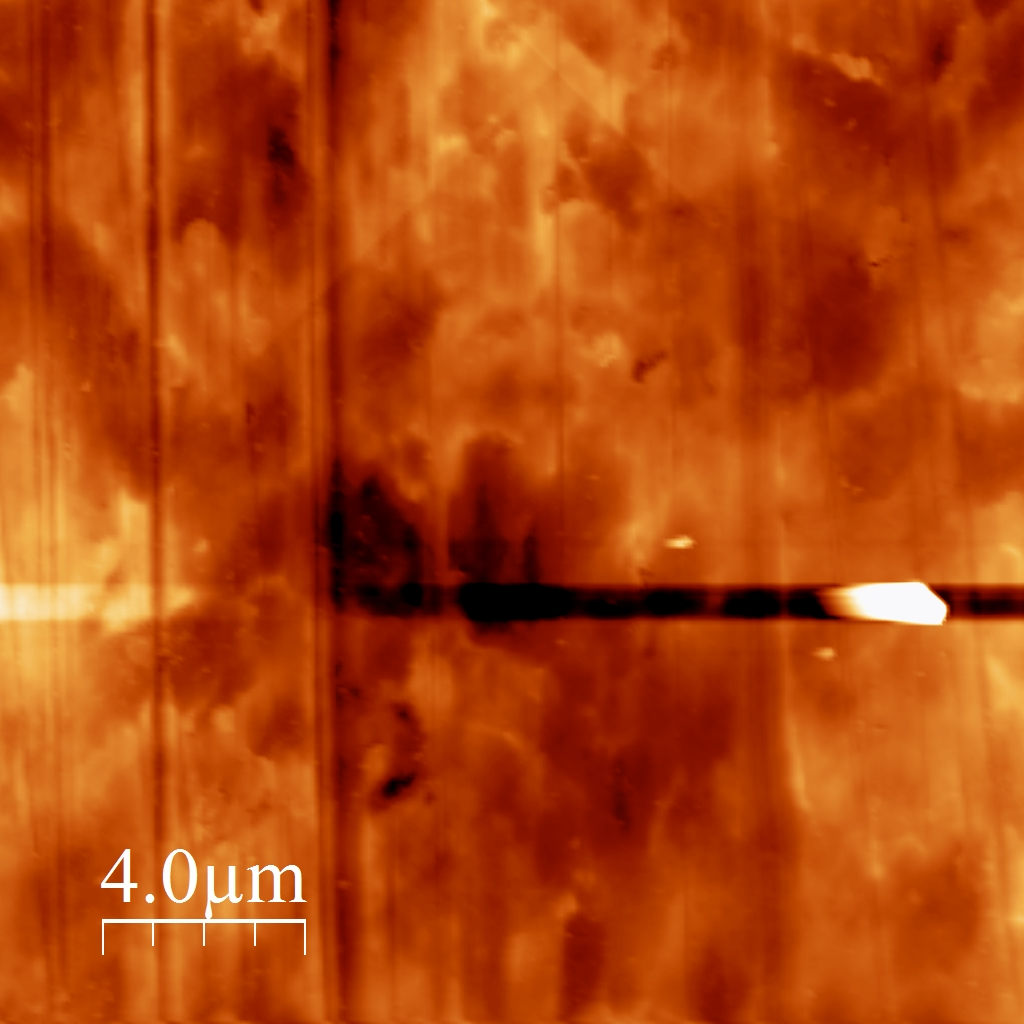
\includegraphics[width=0.4\textwidth]{../Daten/AFM/2015-01-15/as_bought0000.jpg}
 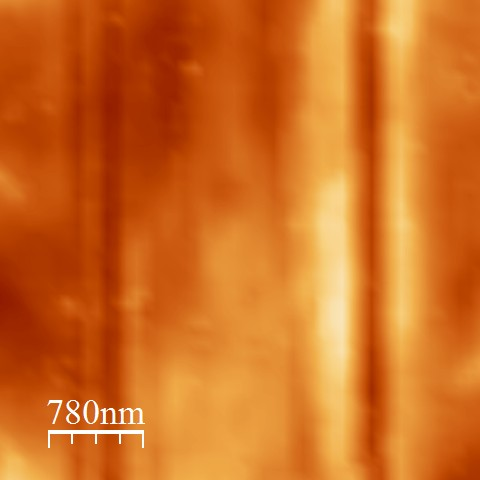
\includegraphics[width=0.4\textwidth]{../Daten/AFM/2015-01-15/as_bought0001.jpg}
 \caption{\SI{0.25}{\mm} as bought from alfa aesar, RMS$\approx$\SI{13}{\nm}, contrast \SI{100}{\nm} ($\approx$ RMS \SI{5}{\nm}, contrast \SI{70}{\nm} in the smaller image)}
\end{figure}
One can see the striations that stem from the production process (from top to buttom).
\begin{figure}[h]
 \centering
 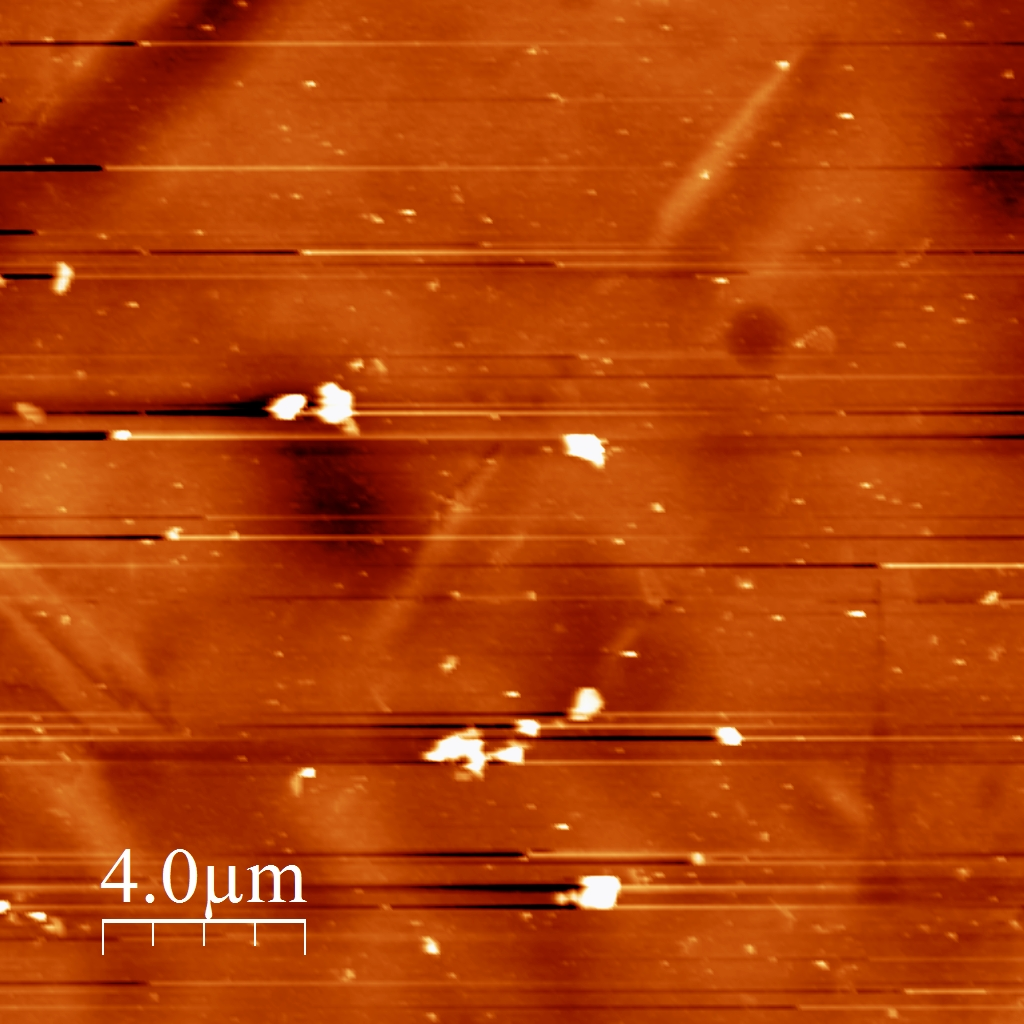
\includegraphics[width=0.4\textwidth]{../Daten/AFM/2015-01-15/polished0000.jpg}
 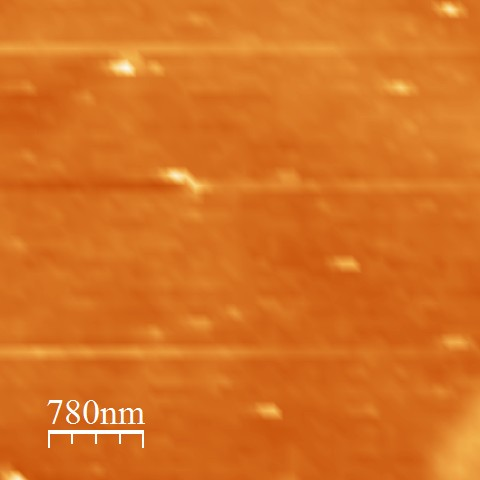
\includegraphics[width=0.4\textwidth]{../Daten/AFM/2015-01-15/polished0001.jpg}
 \caption{\SI{0.25}{\mm} polished 5h in in 75/20/5 phosphoric acid, RMS$\approx$\SI{9}{\nm} in the over all image, contrast \SI{100}{\nm} ($\approx$\SI{5}{\nm} in the smaller image, contrast \SI{70}{\nm})}
\end{figure}
After etching ($U=1.2V$,I=\SIrange{120}{250}{\mA}) \SI{5}{\hour} in a solution \SI{75}{\percent} \SI{20}{\percent} \SI{5}{\percent} (Phosphoric acid, purified water, EG) the striations have gone and the RMS value decreased by \SIrange{30}{45}{\percent} (protrusions due to dirt in the image are counted).
The circular hole is an effect of bubbles in the etching process where the bubble affects the rate of etching. The over all structure changes from a very fuzzy and heterogenous sample height to a flat height contribution with only a little amount of defects. Those are sufficiently seperated in space to exhibit flat regions where the h-BN may grow unperturbated.
\begin{table}
\centering
\caption{Volume and mass fractions for copper foil etching solution.}
\begin{tabular}{lccc}
			&$H_3PO_4$ (85\%)&	EG	&	$H_2O$	\\
Dichte [$g/cm^3$]	&	1.87	&	1.11	&	1.00	\\
$1/rho$			&	0.54	&	0.90	&	1.00	\\
Anteil \%		&	70	&	5	&	25\\
Menge gesamt [$cm^3$]	&		\multicolumn{3}{c}{150} \\
Menge anteilig [$cm^3$]	&	105.00	&	7.50	&	37.50	\\
Gewicht [g]		&	196.35	&	8.33	&	37.50	\\
\end{tabular}
\end{table}

Some foil has been mechanically polished with 4k paper and several hours of Syton polishing. The roughness of these samples has been investigated also in AFM. These are compareable to the chemically polished ones, but are always slightly higher by $\approx 10\%$. Sometimes unwanted new scratches appear after mechanical polish.